\chapter{State of the art}

\label{ch:stateofart}

\section{Human dialogue}
	\subsection{Dialogue acts}
    \label{soa:dialogueacts}
    
        %HK> Les figures issues du Sutton et Barto doivent êtres refaites.
    	%HK> Parler de Clark également : communicative vs. meta-communicative tracks.
    
    	If I say \textit{This dog is big}, I utter a few sounds that can be cast as words. How are these words related to the real objects I refer to? How comes that a sequence of sounds can have effects on others? I can give orders to somebody and make them performs the actions I want as I can congratulate or insult someone and have an emotional impact on her. Also, how comes an utterance can also be judged as a complete nonsense or as a true or false assertion? These are a few questions raised in the philosophy of language.
    
    	In his book called \textit{How To Do Things With Words} \cite{Austin1962}, J.L. Austin focuses on the concept of \textit{speech act} which the title of another book \cite{Searle1969} by John R. Searle, who extended this theory of language. Introducing this concepts is aimed towards bringing answers to the previous questions. Saying \textit{My sister just arrived}, one performs a speech act that can be viewed from different points of view. Suppose that someone is listening as this sentence is being uttered and that person does not speak English, then obviously she only hears a sequence of noises which is the physical, low-level nature of the speech act. When considered from that perspective, the latter is referred to as a \textit{locutionary act}. On the other hand, when the focus is the meaning of the utterance and the message the speakers wants to deliver, the speech act is an \textit{illocutionary act}. Finally, saying something to somebody can have psychological effects on that person: congratulating someone on insulting him can be rewarding or hurting, a strong grounded speech can be convincing...etc... These are referred to as \textit{perlocutionary acts}.
			
			To build a dialogue systems, the traditional approach is to consider the user's and the system's speech acts as illocutionary (rarely perlocutionary) acts. When studying incremental dialogue systems, the \textit{locutionary act} point of view comes at play. In this thesis, this distinction will be clarified.
			
			In the field of psycholinguistics, Herbert H. Clark brings another view of dialogue acts in his book \textit{Using Language} \cite{Clark1996}. The communication channel is split in two tracks, the \textit{communication track} and the \textit{meta-communication track}. The first one is used when the speaker adds new information about the topic of the information whereas the second one is used when she refers to the dialogue itself. For example, saying \textit{OK, I see} or nodding her head are meta-communicative acts. 
        
			In order to guide the user throughout the dialogue, correct potential errors and to confirm some pieces of information, spoken dialogue systems use the meta-communication track. We will see that incremental dialogue opens new possibilities to make an even more subtle use of this track.
        
    \subsection{Turn-taking in human dialogue}
    \label{soa:ttphuman}
    
    	Turn-taking is a sociological phenomenon that is encountered in many different situations: card games, road traffic regulation, CPU resource sharing...etc... In \cite{Sacks1974}, Harvey Sacks describes the social organisation of turn-taking as an economy where \textit{turns are valued, sought or avoided}, depending on the situation at hand. Then, in the rest of his paper, he focuses on the case of human conversation. Obviously, this is subject to many contextual and cultural variations but the objectif of the paper is to meet the challenge of extracting a set of rules that would ultimately describe the human turn-taking mechanisms in a general fashion.
        
        For about six years, Harvey Sacks has been analysing conversation recordings and he came up with a few rules that caracterise human conversation and turn-taking. One of us is particularly interesting given the purpose of this thesis: \textit{transition (from one turn to a next) with no gap an no overlap are common. Together with transitions characterized by slight gap or slight overlap, they make up the vast majority of transitions}.
        
        In \cite{Beattie1982}, a political interview between Margaret Thatcher and Jim Callaghan has been analysed. As a result, the author introduced a classification of turn-taking phenomena where each category is caracterised by the answer to these three questions:
        
        \begin{enumerate}
            \item Is the attempted speaker switch successful?
            \item Is there simultaneous speech?
            \item Is the first speaker's utterance complete?
        \end{enumerate}
        
        %HK> Citer Baumann et Johnsduttir  après Meena...
        Optimising turn-taking means taking the floor at the right time. Humans are very good at detecting the cues for these timings. In artificial dialogue systems, different kinds of features can be used in order to detect these timings \cite{Gravano2011}: prosodic features, lexical features, semantic features...etc... and a lot of work has already been done in this direction \cite{Meena2013}.

        In fact, we even tend to start speaking before the end of our interlocutor's utterance, even interrupting him sometimes. A study led in \cite{Strombergsson2013} reports statistics about times and overlaps in human conversation both directly and over the telephone. Given the type of question that is addressed to the listener, the latter tends to respond more or less quickly, often infering the end of the question and starting to utter the response the answer before its end. In \cite{DeVault2011}, the ability for the machine to replicate that is investigated.

        %HK> Il faut comparer ça aux autres études du genre Beaties1982, le modèle de Raux...
        %HK> Regarder aussi les papiers cités par Raux dans son Finite-State model, dire qu'il utilise les mêmes états que Jaffe et Feldstein.
        In reality, human turn-taking involves even more complicated behaviours resulting in intertwined turns of the speakers. \cite{Raux2009} tries to provide a simple model with very few assumptions. It is a state machine where the following states are considered:

        \begin{itemize}
          \item Only the user speaks.
          \item Only the system speaks.
          \item No one speaks because the user stopped talking.
          \item No one speaks because the system stopped talking.
          \item Both the user and the system speak after a user barge-in.
          \item Both the system and the user speak after a system barge-in.
        \end{itemize}

 In \cite{Wlodarczak2013}, five turn-taking situations are reported:

        \begin{itemize}
           \item \textbf{Within-speaker silence:} The speaker stops for while and then resumes his utterance.
           \item \textbf{Between-speaker silence:} The most intuitive case of turn taking. The speaker stops and after a moment of silence, the listener takes the floor.
           \item \textbf{Within-speaker overlap:} The listener either takes the floor or performs an intervention that is not meant to interrupt the speaker and the latter keeps the floor.
           \item \textbf{Between-speaker overlap:} The listener starts speaking before the end of the speaker's utterance, hence resulting in an overlap and a turn transition.
           \item \textbf{Solo vocalisation:} On person speaks in an unilateral way.
        \end{itemize}
        
        %HK> Parler de la méthode, 12 ans d'études basées sur des enregistrements...
        %HK> Parler des points propices au turn-taking, du principe de minimise gaps and overlaps, thread de recherche basé sur la prosodie.
        %HK> Autres classifications, Beatie1982 et dérivées...
        %HK> Duncan1972 a aussi le mérite d'être cité
				
	\subsection{Incremental speech processing in human conversation}
	

           During a conversation, the listener does not wait for the speaker's utterance to end before trying to understand it. It is processed incrementally and apart from the intuition that we have related to this, a few studies provided convincing arguments supporting the idea. One of the most famous examples is an eye-tracking based study performed in \cite{Tanenhaus1995}. Subjects are given an image to look at through a head-mounted eye-tracking mechanism that records their eye-gaze at a millisecond scale. Then, ambiguous and unambiguous sentences were uttered, for example:

           \begin{itemize}
             \item \textbf{Ambiguous version:} Put the apple on the towel in the box.
             \item \textbf{Unambiguous version:} Put the apple that is on the towel in the box.
           \end{itemize}

           For this example, when the users are provided with an image of an apple on a towel, a towel with nothing on it and box, their eye-gaze show different patterns depending on which version of the utterance they listen to. In the ambiguous case, they tend to start by looking at the apple, then to the towel with nothing on it, then to the apple again and finally at the box. In the unambiguous case, they directly look at the apple and then to the box. Most importantly, these movements happen as the sentence is uttered.

           This is also pretty much related to the garden path sentence effect. Consider the following sentence (taken from the related Wikipedia article): \textit{the government plans to raise taxes were defeated}. Most people feel the need to read it twice or even several times before understanding its meaning. When one starts reading \textit{the government plans to raise taxes}, she automatically understands that taxes are planned to be raised by the government but then comes the disturbing end of the sentence \textit{are defeated}. The only solution is to parse \textit{plans} as a noun and not as a verb. This is also an argument in favour of human incremental processing.

           Finally, when humans are reading a text, they tend to skip a few words with no loss of the meaning. In \cite{Ilkin2011}, the authors show that we are able to predict a few words while reading given the context and the sentence structure (eye-traking has also been used here). For example, when the readers reach the sentence \textit{The worker was critised by his boss}, the word boss seems to be guessed ahead of time, again supporting the idea of incremental speech processing.


\section{Spoken dialogue systems and incremental behaviour}
    
	\subsection{Spoken dialogue system}
        \label{soa:sds}
        
%HK> Citer papier SIGDIAL 2014 juste après companionship.
	A spoken dialogue system (SDS) is an automated application that interacts directly with a human being in natural language. Virtual assistant like Siri (Apple) or Cortana (Microsoft) are good examples of SDSs. They are task-oriented as their goal is to help to user to achieve some task. There also exist a few SDSs that are only used for chatting and companionship.
	
	Traditional computer interfaces are presented in the form of controls in an application (text boxes, buttons) or web pages. They are heavily used and they have been proven to be efficient enough, providing an accurate way of human-machine interaction. So, why building spoken dialogue systems? What are the advantages of the vocal modality?
		
	An obvious motivation for building spoken dialogue systems is the thrive for human-likeness. In \cite{Edlund2008}, an interesting analysis of the way humans perceive dialogue systems they are interacting with is performed. These systems are complex and humans keep a simplified representation of them during the interaction (called metaphors in \cite{Edlund2008}). Two of them are the most common:
	
	\begin{itemize}
		\item \textit{Interface metaphor:} The system is viewed as an interface just like non dialogue-based systems. Users adopting this representation of the system tend to use vocal commands instead of complete sentences. Moreover, they tend to keep silent when the system tries to behave like a human, by saying \textit{Hi!} for example.
		\item \textit{Human metaphor:} In this case, the users tend to view the system as a real human, therefore adopting a more natural way of communication. These users generally have higher expectations of the system's ability to answer their requests as well as it ability to perform human-like turn-taking actions.
	\end{itemize}
	
	Nevertheless, it is also legitimate to ask the question whether human-likeness should be a goal in the conception of dialogue systems of not. In \cite{Edlund2008}, four kinds of objections to pursuing that goal are discussed. The first one is the feasibility: is there any hope that someday, we will be able to build systems that behave exactly like humans. This have raised huge debates during the last decades. The second question is utility: do we really need systems that imitate humans? Apart from the fact that it would help us to better understand the way we communicate, it is easy to justify in the case of some applications like companionship and entertainment. It is less obvious when it comes to task-oriented dialogue. The third point is related to the concept of \textit{uncanny valley} \cite{Mori1970}: as machine's human-likeness increases, they reach a point where they start becoming annoying for the user. Nevertheless, by bringing even more improvements, we can cross this valley and come up with human-like solutions that no longer have such problems. Finally, the last question brought up in \cite{Edlund2008} is the one of symmetry. If machines have a similar behaviour to humans, then users are likely to push the human metaphor to the limit by unconsciously thinking that machines really understand what they are saying, thus expecting more complex reactions like the ones due to emotions for example.

        %HK> Références?
        The multiplication of services and support platforms in modern society engenders huge costs that dialogue systems can help to reduce. By analysing client paths while demanding assistance from an expert, it is possible to identify commonly asked questions and recurrent patterns. By gathering such information, it is also possible to design dialogue systems that can interact with users and respond to their requests without any human intervention (of course, in the case the interaction fails, the client is redirected to a normal service platform). This can dramatically reduce service and support costs and also improve the quality of service as it is accessible any time, with no interruptions (unlike real platforms that are more often open at working time only). Moreover, when a client calls, the answer is immediate and her call is no longer queued causing waiting time (which she pays for) with sometimes no answer at all.

	%HK> Rajouter d'autres exemples que Amazon Echo.
	With the development of the Internet of Things (IoT) during the last few years, new human-machine interactions can be imagined. For instance, the concept of \textit{Smart Home} is currently making its enter in the marker of Artificial Intelligence through the contributions of several companies and start-ups: Amazon Echo... In this context, the advantage of speech communication is clearly relevant as it is hands and eyes-free. The user can command her house from any room with no extra device needed. In some situation, her hands are already occupied by some other task. For example, she can be cooking \cite{Laroche2013} while asking \textit{What should I put next in my salad?} or \textit{Can you add milk to my errands list please?}.

        %HK> Citer papiers sur le companionship.
        Finally, talking agents and talking robots can also be designed for entertainment and companionship. The vocal modality is the most natural way of interaction and therefore, it is very useful in this area.

		
		\begin{figure}
			\centering
			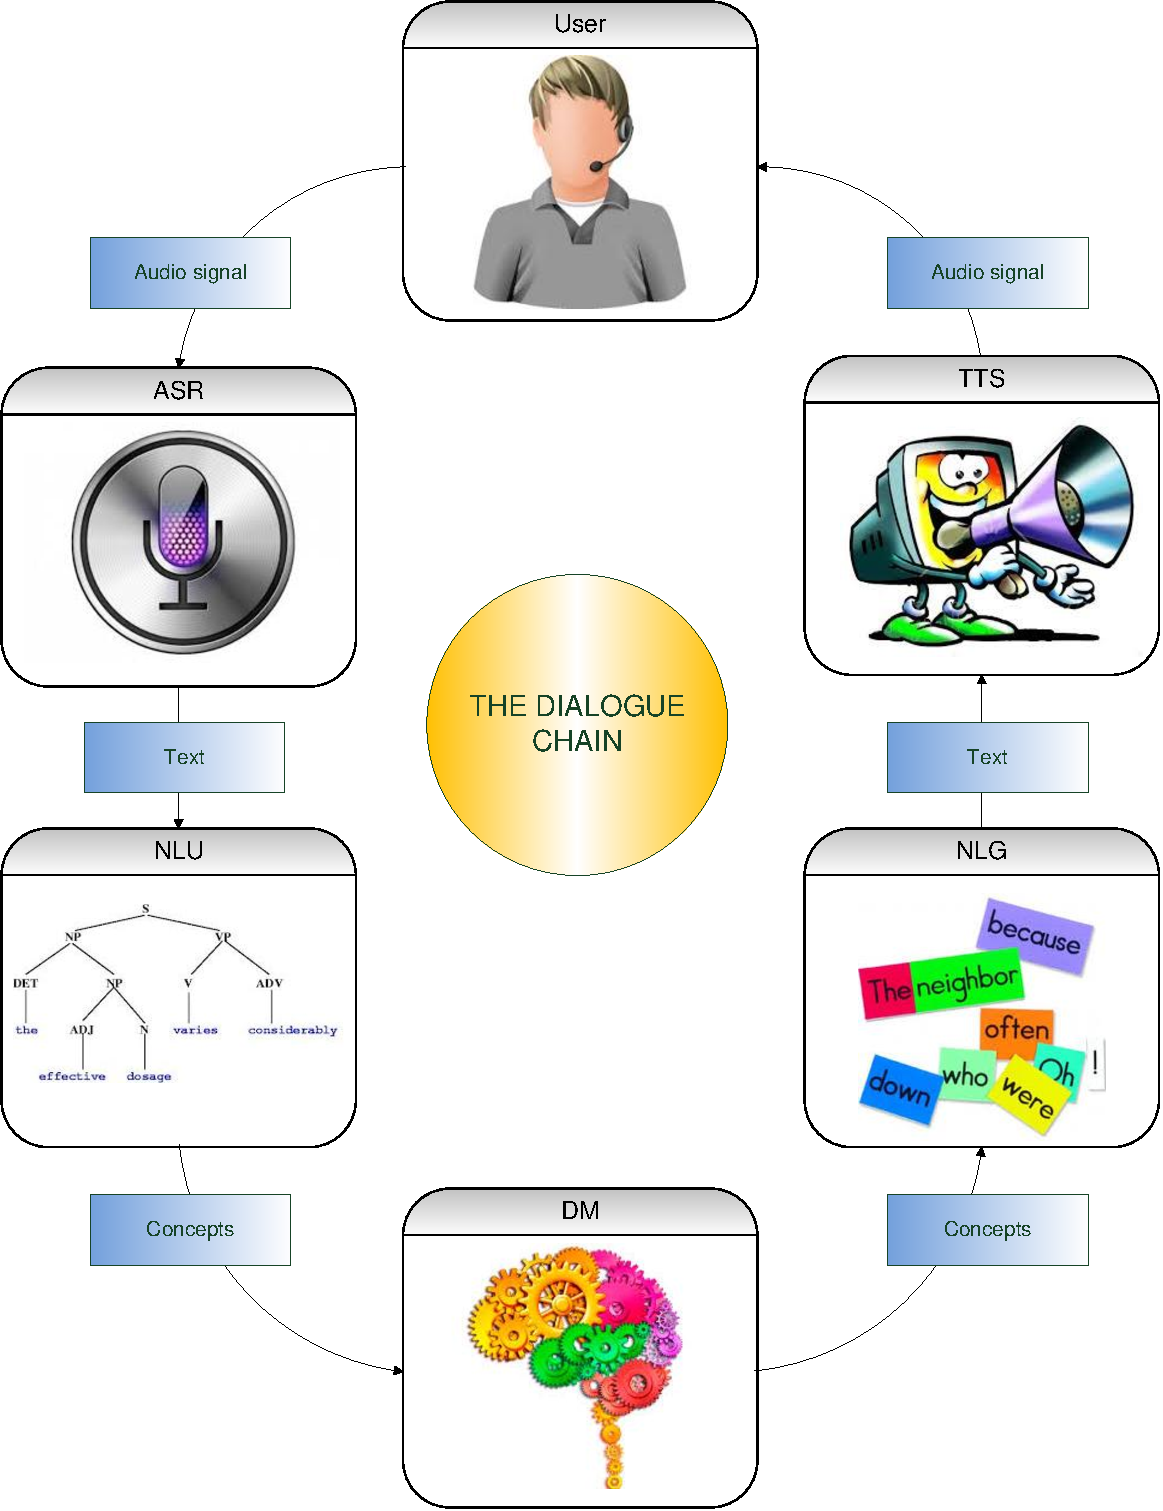
\includegraphics[scale=0.8]{figures/DialogueChain.pdf}
			\caption{The dialogue chain}
			\label{fig:dialchain}
		\end{figure}

		The classic architecture of an SDS is made of five main modules (Figure \ref{fig:dialchain}):
		\begin{enumerate}
			\item Automatic Speech Recognition (ASR): transforms the user's audio speech signal into text.
				\item Natural Language Understanding (NLU): outputs a conceptual representation of the user's utterance in text format.
				\item Dialogue Manager (DM): given the concepts extracted from the user's request, a response (in a conceptual format too) is computed.
				\item Natural Language Generation (NLG): transforms the concepts computed by the DM into text.
				\item Text-To-Speech (TTS): reads the text outputted by the NLG by using a synthetic voice.
		\end{enumerate}

		%HK> Rajouter des références.
		Speech recognition technology is an old problem with long history. During the 1950s, a group of researchers from Bell Labs developed the first technology that is able to recognise digits from speech (in fact, speech perception has been under study since the early 1930s). Then, during the second half of the last century, new advances have made it possible to build ASR solutions with larger vocabulary and with no dependence on the user. In the 1960s, Hidden Markov Models (HMMs) were proved to be useful for speech recognition and they were the most popular technique two decades later. Commercial products using ASR technology had to wait until the 1990s to be finally released in the marked as they reached and interesting vocabulary (even though their accuracy and their delay were far behind the technology we have today). Performances kept improving incrementally until 2009, when Deep Learning algorithms were tested; the Word Error Rate (WER) decreased by 30\%. During the last six years, research continued in that direction giving birth to accurate and reactive speech recognition solutions (Google, Nuance, Sphinx, Kaldi...). Therefore, ASR is no longer a bottleneck in the development of spoken dialogue systems, and as we will see later, the delays they offer make it possible to design reactive incremental dialogue systems. Commercial off-the-shelf ASR solutions like Google ASR or Nuance products are able to recognise almost every word in many languages, including named entities. Finally, the ASR output is not only the text that the recognition algorithm figures out to be the best match for the input audio signal, but a list of the N most likely hypotheses and the corresponding confidence scores: it is called the N-Best. For instance, an 5-Best could be:

		\begin{itemize}
			\item 0.965: I would like to book a flight from New-York to Los Angeles
			\item 0.931: I could like to book a flight for New-York to Los Angeles
			\item 0.722: Cold like a book fly New-York to Los Angeles
			\item 0.570: Cold like look flight pork to Los Angeles
			\item 0.441: Cold bike look fly New-York to Los Angeles  
		\end{itemize}

		%HK> Référence sur Rule-based vs. statistical-based? Un survey sur la NLU?
		The scope of NLU technology is a sub-field of Natural Language Processing (NLP) whose scope much wider than the spoken dialogue field. Since the 1950s, researchers have been trying to develop several models and ontologies in order to automatically process natural language with several applications in sight: topic recognition, sentiment analysis, news filtering and analysis, natural speech processing...etc...The ambition manifested during 1950s and the early 1960s quickly had to face reality as the expected objectives were far from being reached. As a consequence, research in this area was significantly slowed down between the 1960s and the 1980s. During the last decade, NLP research has found a second wind thanks to new Machine Learning, bringing them at the heart of lucrative businesses like recommendation and digital marketing. NLU refers to the set of techniques in order to make the machine understand the underlying structure of a text in natural language. To do so, a lexicon as well as an ontology (concepts and the links between them in a specific domain) should be built. Existing dialogue systems are able to interact with the user in the domain they are built for only, however, during the last few years, researchers have been pushing the boundaries of open-domain systems \cite{Gasic2013}. Therefore, earlier NLU solutions are based on a set of handcrafted parsing rules, however, new statistical-based models have been proven to be more robust and easy to generalise over domains.

		%HK> Faire un choix: "reinforcement learning", "Reinforcement Learning" ou "RL". Idem "spoken dialogue systems", "Spoken Dialogue Systems" ou bien "SDSs".
		%HK> Autres références pour le DSTC, RNN de Hendersen...etc...
		Dialogue Management is at the heart of Spoken Dialogue System's current research. A couple of decades ago, for the first time, dialogue has been modeled as Markov Decision Processes (MDPs) problem, hence being solved using reinforcement learning \cite{Eckert1997}. The dialogue state is generally defined by the whole dialogue history and the set of actions in each state are the dialogue acts that the system can make. In 2007, in order to represent the uncertainty over the user's intent (due to ASR or NLU imperfections), dialogues have been cast as Partially Observable Markov Decision Processes (POMDPs) \cite{Williams2007}. This gave raise to the notion of \textit{believe tracking} which objective is to keep a distribution over the possible user intents. In order to encourage research in that direction, a Dialogue State Tracking Challenge (DSTC) has been launched a few years ago \cite{Williams2012b}, bringing new contributions each year. This approach has been shown to provide interesting results, however, the size and the dimensionality of the state space makes it intractable most of the time.

		%HK> Noms de startups et de boites faisant de la génération de texte automatique?
		The NLG task is the inverse of the NLU one. It started being used in the 1990s for purposes like financial news summary. A few start-ups and big companies also provide automatic text generation solutions that are used to quickly produce reports or official letters. The main challenge for such systems is to be able to generate a variety of different words, expressions and sentences in order for them not to be repetitive and for the result to be as realistic as possible. This is even more crucial when it comes to dialogue systems as they are supposed to simulate a real conversation with the user which is a highly variable task).

		During the 1930s, Bell Labs were not only interested in ASR but they also developed a new approach for the inverse task: the TTS (also known as \textit{speech synthesis}). The human speech is broken into small acoustic components that are sequentially pronounced by the system. They built the first machine demonstrating this mechanism: the Voder. As far as this task is concerned, the challenge for the system is to sound as human-like as possible, in terms of phoneme transitions, speech rate and prosody. Even though substantial advances have been accomplished since the Voder, it is still easy to distinguish between a synthesised and a real human voice.

		%HK> Parler du test de Turing comme test ultime?

        \subsection{Dialogue systems evaluation}

                In this section, we focus on the question of dialogue systems' evaluation. What makes a dialogue system better than another one? What metrics should be taken into account while evaluating dialogue systems? What are the most important characteristics of dialogue systems that should be improved?

                %HK> Références pour PARADISE.
                In the PARADISE framework, a distinction is made between two kinds of metrics that are usually used for evaluating dialogue systems: objective and subjective metrics. The first category contains all the Key Performance Indicators (KPIs) that can be measured by an algorithm by accessing the dialogue logs only, whereas the second one is made of the users's appreciations of the dialogue quality or specific characteristics like reactivity or human-likeness.

                %HK> Est-il possible de justifier de façon plus propre la correlation entre la duration et la task completion.
                Objective metrics that are commonly used are the dialogues' mean duration and the task completion ratio. Generally speaking, these two metrics are correlated as the user gets impatient when the dialogue lasts for too long (even the user can get impatient for other reasons, like the repetition of the same system's dialogue act several times). Moreover, the user's speech rate and the way they communicate introduces some variability when using these metrics. Finally, it is legitimate to ask ourselves: do we really want shorter dialogues? First, this depends on the type of dialogue system at hand. If it is designed for entertainment or companionship, then there is no need for seeking faster dialogue strategies. However, in the case of task-oriented dialogue, looking for shorter dialogues makes sense as a measure of efficiency.

                %HK> Citer Layla sur l'Ordinal Regression.
                Subjective metrics are generally gathered using a survey at the end of each dialogue. Several metrics can be collected this way: the global quality of the dialogue, naturalness/human-likeness, reactivity...etc...However, this also raises the problem of variability between users. Most often, they are asked to evaluate the system on a likert scale (1 to 5 or 1 to 10), but a user answering 4 could be equivalent to another user answering 3 or 5. Therefore, the absolute evaluation is less significant than the relative one given a specific user.

	\subsection{Incremental dialogue systems}
    
		%HK> Pour Levelt, citer le livre au lieu de la review.
		The idea of incremental systems goes back to incremental compilers \cite{Lock1965}. An incremental compile processes each new instruction independently from the previous ones. In his book \textit{From intention to articulation} (1989), Levelt analyses the mechanisms underlying the way humans formulate their ideas in natural language. The approach is closer to computational linguistics than psycholinguistics. The second part of the dialogue chain (DM, NLG and TTS) are analysed using a different terminology: the \textit{Conceptualizer}, the \textit{Formulator} and the \textit{Articulator}. Therefore, a local modification of the code does not affect the whole result of the compilation. The idea of processing natural language in an incremental way is first introduced in \cite{Wiren1992} according to \cite{Kilger1995}. Instead of feeding modules with complete utterances, the input is pushed chunk by chunk (500ms of audio signal, one word of a sentence...etc...) making the output change several times before the end of the user's utterance.

		Currently deployed dialogue systems have a simple and rigid way of managing turn-taking. The interaction mode they offer is similar to a walkie-talkie conversation as the system waits for the user to finish her utterance before taking the floor and vice-versa (even though some systems allow the user to interrupt the system). Such systems will be referred to as \textit{traditional dialogue systems} in this thesis.

		%HK> Retrouver le papier sur la lecture et l'incrémental et le citer avec Tanenhaus.
		%HK> Rajouter Beatie1982 dans le bibtex et le citer dans ce paragraphe juste après barging-in. Retrouver le papier qui a repris Beatie1982 et le citer avec lui.
		In human to human conversation, the listener does not wait for the speaker to finish his sentence before processing it; it processes it as it is spoken \cite{Tanenhaus1995}. As a consequence, human beings perform a large panel of turn-taking behaviours while speaking, like backchanneling (\textit{aha}, \textit{yeah}...) or barging-in.
	
		To replicate this behaviour, a new generation of SDSs has been the focus of current research for a few years. An SDS is said to be incremental when it is able to process the user's speech on the fly. The input signal is divided into small chunks and the growing sentence is reprocessed at each new chunk \cite{Schlangen2011}. Table \ref{tab:incrnluex} gives an example illustrating the functioning of an incremental NLU module (in a hotel room booking service). For the sake of simplicity, processing delays are neglected.
	
		\begin{table}[th]
			\vspace{2mm}
			\centerline{
				\begin{tabular}{|l|l|l|}
					\hline
					\textbf{Time step} & \textbf{NLU input} & \textbf{NLU output} \\
					\hline
					1 & I & empty \\
					\hline
					2 & I won't & empty \\
					\hline
					3 & I would & empty \\
					\hline
					4 & I would like to & empty \\
					\hline
					5 & I would like to cook a & empty \\
					\hline
					6 & I would like to book a room & \textbf{action:} BOOK \\
					\hline
					7 & I would like to book a room on May & \textbf{action:} BOOK \\
					\hline
					8 & I would like to book a room on May 7$^{th}$ & \textbf{action:} BOOK \\
					& & \textbf{date:} 05-07 \\
					\hline
					9 & I would like to book a room on May 7$^{th}$ and I will & \textbf{action:} BOOK \\
					& & \textbf{date:} 05-07 \\
					\hline
					10 & I would like to book a room on May 7$^{th}$ and I will & \textbf{action:} BOOK \\
					& be driving & \textbf{date:} 05-07 \\
					& & \textbf{parking:} YES \\
					\hline
				\end{tabular}
			}
			\caption{Taxonomy labels}
			\label{tab:incrnluex}
		\end{table}

	\subsection{Advantages of incremental processing}
						
		%HK> Human-likeness: Edlund2008
		%HK> User satisfaction in general: Aist2007, Skantze? Selfridge?
		%HK> Reactivity
		%HK> Limit desynchronisations
		%HK> Efficiency, inciting the user to formulate more focused requests : Ghigi2014, Khouzaimi2015, Tiancheng2015
		%HK> Multimodality : Fink1998, voir du côté de Bohus, Matthias2009

                Before discussing the different reasons why incremental processing should be preferred to rigid turn-taking, it is important to note that a few studies led with real users have shown that incremental dialogue systems offer a better user experience. For instance, in \cite{Aist2007}, an ordinal regression has been performed between the user satisfaction and several features with a flag for incremental processing among them. A significant correlation between incremental processing and the global user satisfaction has been found.

                As discussed in Sect. \ref{soa:sds}, human-likeness is a legitimate goal for dialogue systems (at least worth trying). When talking to each other, humans perform a rich set of turn-taking phenomena (see Sect. \ref{soa:ttphuman}) and in spite of the fact that they do not talk in a rigid walkie-talkie manner, they manage to maintain to avoid desynchronisations and to keep a conversation that is going forward. Replicating these behaviours from the machine's point of view can therefore be interesting. We might expect that the user feels more at ease while using a more human turn-taking mode hence keeping the human metaphor even further.

                The other aspect that is interesting about incremental dialogue is reactivity. As the system processes the user's request before its ends, it is possible to design accurate end-point detection in order to detect the end of this request as soon as possible \cite{Raux2008}. Moreover, incremental dialogue systems can interrupt the user to report a problem, like in the following example:
								
								\begin{dialogue}
									\speak{USER}{I would like to book a room for tomorrow with ...}
									\speak{SYSTEM}{Sorry, we are full tomorrow.}
								\end{dialogue}
								
								This can help the user get to her goal faster but one should be very careful about the way it is implemented as there is a risk that user interruption actually harms the user experience (event though the intent is to go faster, see Sect. \ref{soa:challengesincr}). Nevertheless, a corpus study led in \cite{Ghigi2014} showed that when users are interrupted, they tend to adopt a more sober way of expression, hence directly increasing the dialogue efficiency and indirectly as the risk of misleading off-domain words and expressions is reduced \cite{Ghigi2014,Khouzaimi2015b,Zhao2015}.
								
								Early barge-in both from the user and the system's side is also a way to limit desynchronisations. An example of a desynchronised dialogue could be:
								
								\begin{dialogue}
									\speak{USER}{01 45 38 37 89}
									\speak{SYSTEM}{01 45 28 37 89}
									\speak{USER}{No, not 28 but 38}
									\speak{SYSTEM}{Sorry, you mean 28 38}
									\speak{USER}{What?}
									\speak{SYSTEM}{28 38 1}
								\end{dialogue}
								
								In this example, the user could have reported the mistake earlier if he could barge-in:
								
								\begin{dialogue}
									\speak{USER}{01 45 38 37 89}
									\speak{SYSTEM}{01 45 28...}
									\speak{USER}{No, 38}
									\speak{SYSTEM}{Ok. 01 45 38}
									\speak{USER}{31 89}
									\speak{SYSTEM}{31 89}
								\end{dialogue}
								
		Another interesting aspect about incrementality is that it can leverage multimodal dialogue systems. In fact there are two aspects of multimodality and they can both benefit from incremental processing:
								
		\begin{itemize}
		   \item \textbf{Input multimodality:} Most researchers in the community refer to this aspect when talking about mutimodal systems. A system input can be multimodal in the sense that it can handle speech input, but also text, gesture or eye-gaze for example. The main challenge faced by this kind of setup is the problem of mixing these inputs in order to make the inference of the user's utterance. In the case of multimodal systems, the world is considered as a flow of information coming from multiple sources of information. The different modalities are not necessarily sampled with the same rate nor support the same delays, therefore, it is important to find convenient ways to synchronise them.
		   \item \textbf{Output multimodality:} The machine can also use different channels of information while communicating. For example, the speech modality can be used at the same time as a moving avatar with facial expressions. It can also be coupled with the input multimodality paradigm to create highly interactive interfaces like \cite{Johnston2014}.
		\end{itemize}

                On the one hand, in the case of input multimodality, incremental processing can help process the different flows of information more quickly hence producing more reactive systems that are more aware of their environment. On the other hand, systems operating in an output multimodality way can also be leveraged using incremental behaviour as the different modalities can be used to provide a richer real time feedback to the user, like an avatar that frowns or nods its head while not understanding or agreeing for example.


	\subsection{New challenges raised by incremental dialogue processing}
	\label{soa:challengesincr}
    
		%HK> Citer Dan Povey pour Kaldi.
		The first problem to consider when talking about incremental spoken dialogue systems is the question of ASR \textit{latency}, which is the time needed by the recognition algorithm to provide the text output corresponding to an audio signal. As we said earlier, the ASR accuracy has been a bottleneck in the development of spoken dialogue systems for many years but thanks to recent advances in this field, it is no longer the case. Similarly, incremental dialogue systems require quick responses from the ASR and the delays needed but speech recognition modules have been too long for many years which was a limiting factor in the development of incremental dialogue systems. However, in the last few years, ASR technology has became reactive enough \cite{Platek2014}. Nevertheless, it is important to be aware that there is a tradeoff between the accuracy and the vocabulary size on one hand and the latency on the other hand. Kaldi, which is an ASR solution designed by researchers (and which is mostly used by them), makes it possible to design one's own acoustic and language model as well to set one's own parameters in order to control this tradeoff. On the other hand, more off-the-shelf solutions like Google ASR do not give the user such possibilities (however, accuracy and delays are well balanced for most applications).

		%HK> Citer Ethan et Jason au sujet de l'instabilité si ce n'est déjà fait.
		If we observe the successive partial results of an incremental ASR module during a user's utterance, it is likely that the progression they follow is not monotonous. In other words, a partial result is not guaranteed to be a prefix of results to come. The following example showing successive ASR results illustrate this phenomenon:

		\begin{enumerate}
			\item Euh
			\item I
			\item Euh good
			\item iPod
			\item I would
			\item I good bike
			\item I would like
		\end{enumerate}

		This phenomenon is called ASR \textit{instability} (or stability depending on the sources) \cite{Selfridge2011}. This factor is also related to the tradeoff between latency and accuracy as preferring fast ASR over accurate ones can lead to very unstable results (the system is not given enough time to check that its results are accurate, thus ending up delivering wrong partial results most of the time), and the vice versa.
		
This leads to one of the main challenges raised by incremental processing: the ability to \textit{revise} the current hypothesis. All the modules in the dialogue chain are impacted by this problem. As an illustration, suppose that the user interacts with an incremental personal assistant on her phone and makes the following request \textit{Please call the number 01 45 80 12 35}. The last digit is first understood as being 30 and then 35, therefore, if the system is too reactive, there is a risk that it starts calling the wrong number and maybe start uttering the sentence \textit{Ok, calling 01 45 80 12 30}. Afterwards, the system understands 35 instead of 30 hence needing a correction mechanism in order to stop the TTS, to cancel the call, to perform a new one and to provide a new answer to the user. Nevertheless, even though the system at hand is equipped with such a mechanism, using it very often is not an optimal way of managing incremental input as it causes extra delay as well as non-natural behaviour (stopping the TTS and starting again with another utterance). This introduces a similar tradeoff to the one discussed for the ASR module but from the DM perspective: if decisions are taken too quickly, it is likely that some of them are wrong hence activating the correction mechanism. On the other hand, if the DM is slow to take action, then it lacks reactivity and there is no point for it to be incremental. As a consequence, it is important to determine the right moment to commit to the current partial utterance and to take action based on it \cite{Raux2008,Lu2011}. This constitutes the main objective of this thesis.

		Incremental NLG also raise new problems which are illustrated in \cite{Baumann2013}. In this paper, a system has to describe a car's trajectory in a virtual world. When the latter approaches an intersection where it has to turn right or left (no road straight ahead), then the system utters something like \textit{The car drives along Main Street and then turns...euh...and then turns right}. In this example, the system is sure that the car is going to turn which makes it possible for it to commit to the first part of the sentence with no risk. However, this is not always the case as a new chunk of information from the user can change the whole system's response. In this thesis, the NLG is not incremental as we consider that the DM's response is computed instantly at each new micro-turn (event though it is not necessarily stable and it can vary from micro-turn to micro-turn). Finally, in purely vocal applications, computing the NLG results incremental does not make much sense as the user's and the system's utterances do not overlap most of the time \cite{Sacks1974}. However, this is an interesting behaviour as far as multimodal applications are concerned.

		%HK> Trouver des références pour ce paragraphe et bien le justifier (le papier de Baumann parle-t-il de ça aussi?).
		Building an incremental TTS module can also be very tricky. In order for the synthetic voice to be the most human-like as possible, prosody should be computed accurately and to do so, the sentence's structure and punctuation have to be taken into account. This information is no longer given in the case of incremental TTS or it arrives too late.


	\subsection{Existing architectures}
		\subsubsection{Sequential paradigm}
			
			A general abstract model of incremental dialogue systems has been introduced in \cite{Schlangen2011}. In this approach, the dialogue chain is maintained and each one of the five components is transformed into its incremental version. We will refer to this view of incremental dialogue systems as the \textit{sequential paradigm}.
				
			Each module is composed of three parts, the Left Buffer (LB), the Internal State (IS) and the Right Buffer (RB). As described in Section \ref{soa:sds}, each module is also characterised by the type of input it processes as well as the type of output it computes. In incremental dialogue, all these data flows have to be divided into small chunks which are called Incremental Units (IU) \cite{Schlangen2011}. For example, the audio signal that is given as an input to the ASR module can be divided into 500ms chunks that are processed one by one. Each IU is first added to the LB, then it is taken by IS for processing and once a result is available, a new IU of a new kind is outputted in the RB. As the RB of one module if the LB of the following one in the dialogue chain, the data propagation through the dialogue system is insured.
			
			It is important to note that a new IU in the LB does not necessarily imply that a new IU will be pushed into the RB on top of the ones that already existed there. An example given in \cite{Schlangen2011} is the following: suppose the user utters the number \textit{forty} which processed incrementally, then first the ASR outputs \textit{four} and then \textit{forty}. As a consequence, the second hypothesis does not complete the first one but it cancels it. This phenomenon will be discussed more in details in Chapter \ref{ch:simulation}.
			
			Adopting this paradigm is a natural way of enhancing traditional dialogue systems with incremental capabilities. It is interesting from a computational and design point of view as the different tasks are separated. Therefore, one is able to evaluate the different components independently \cite{Baumann2011} and have a global view on which area still needs improvement.

		\subsubsection{Multi-layer paradigm}
		
			The problem of dialogue management in traditional dialogue systems can be formulated as follows: at each dialogue turn, given the dialogue context (including the last user's utterance), what is the right dialogue act to perform? In the incremental frame, this definition no longer holds as dialogue acts are no longer attached to dialogue turns. Therefore, one way to tackle the problem is to split the dialogue management task in two components, the high-level and the low-level handlers. This paradigm is directly motivated by Austin's, Searl's and Clark's contributions discussed in Section \ref{soa:dialogueacts} as the high-level module handles illocutionary acts (the communicative track) whereas the low-level one manages locutionary acts (the meta-communicative track).
				
				%HK> Citer Pickering and Gravano 2003?
				As reported in \cite{Lemon2003}, this approach is more in alignment with results in the psycholinguistic field. The phenomena observed in the meta-communicative track are complex, and the interaction happen on multiple levels, not always following the classical dialogue chain. Having a separate module for handling these phenomena is therefore a more natural paradigm.
				
				Switching from the traditional dialogue management approach to the incremental one is also a transition from discrete time to continuous time, from a synchronous to an asynchronous processing \cite{Raux2007}. The low-level module is continuously (approximated by a high frequency processing in computers) listening to the outside world and waiting for events that might be interesting to communicate to the high-level handler. On the other hand, the latter communicates actions (dialogue acts) and it is the role of to the low-level module to choose whether to retrieve them to the user or not as well as choosing the right moment in case it decides to speak.
				
				Finally, starting from a traditional dialogue system, it is more easier and straightforward to transform it into an incremental one if one adopts this paradigm. Adding an extra low-level module to the dialogue manager is enough \cite{Selfridge2012a,Khouzaimi2014a}. At each new incremental input, this module sends the whole partial utterance from the beginning of the current turn to the dialogue manager and gets its response. Based on that and eventually some other features, it decides whether to take the floor or not. As most of the requests sent to the dialogue manager are "fake" as they are not meant to be acted on, they should not affect the dialogue context. Therefore, whether multiple instances of the dialogue manager are used, whether the dialogue context is saved and restored at each new request, unless the low-level module decides to take the floor.

\section{Reinforcement Learning}
	\subsection{Definition}
    
    	%HK> Insérer une image représentant l'interaction entre l'agent et l'environnement et s'y référer dans ce paragraphe.
        %HK> Remplacer tous les $$ par des eqnarray.
    	Reinforcement Learning (RL) is a sub-field of machine learning where an agent is put into an environment to interact with, and figure out through the process of \textit{trial and error}, what the best actions to take are, given a reward function to maximise \cite{Sutton1998} (see Fig. \ref{fig:rlscheme}).
        
        \begin{figure*}[ht]
          \centering
          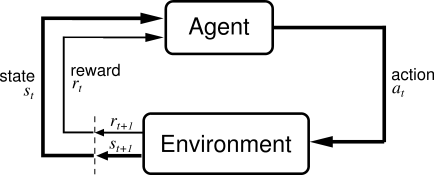
\includegraphics[scale=0.8]{figures/RL.png}
          \caption{The interaction between the agent and the environment in reinforcement learning}
          \label{fig:rlscheme}
        \end{figure*}
        
        Formally, the agent is cast as a Markov Decision Process (MDP) which is a quintuple $\mathcal{M} = (\mathcal{S},\mathcal{A},T,R,\gamma)$ where:
        \begin{itemize}
        	\item $\mathcal{S}$ is the \textit{state space}. At each time step $t$, the agent is in some state $s_t \in \mathcal{S}$.
            \item $\mathcal{A}$ is the \textit{action space}. At each time step $t$, the agent decides to take action $a_t \in \mathcal{A}$.
            \item $T$ is the \textit{transition model}. It is the set of probabilities $\mathbb{P} (s_{t+1} = s'|s_t = s)$ for every $(s,s') \in \mathcal{S}^2$.
            \item $R$ is the \textit{reward model}. If $r_t$ is the immediate reward due to taking action $a_t$ in state $s_t$, then $R$ is the set of distributions of $r_t$ for every $(s_t,a_t) \in (\mathcal{S},\mathcal{A})$.
            \item $\gamma \in [0,1[$ is referred to as the \textit{discount factor}. In the RL framework, the aim of the agent is not to maximise the immediate reward but the \textit{expected return}, where the return $R_t$ is defined as follows:
            
            $$ R_t = r_{t+1} + \gamma r_{t+2} + \gamma^2 r_{t+3} + ... = \sum_{k=0}^\infty \gamma^k r_{t+k+1} $$
            
            Therefore, when $\gamma = 0$, the agent maximises the immediate reward only and when $\gamma$ tends towards 1, the agent maximises the sum of all the future rewards. More generally, the parameter $\gamma$ controls how far-sighted is the agent in terms of future rewards.
		\end{itemize}
        
        A \textit{policy} $\pi : \mathcal{S} \rightarrow \mathcal{A}$ is a mapping between the state space and the action space. An agent is said to follow the policy $\pi$ when for each time $t$, it takes the action $a_t = \pi(s_t)$. A policy can also be stochastic, in which case, $\pi (s,a)$ denotes the probability of choosing action a when the agent is at state s. A key aspect of MDPs is the \textit{Markov property}. Being at state $s$ is the only information necessary to predict the future expected return, and no information about the past is necessary. Therefore, given a policy, each state $s \in \mathcal{S}$ is given a value $V^\pi (s)$ which is the expected return for being at this state and following the policy $\pi$ afterwards:
        
        	$$ V^{\pi} (s) = \mathbb{E} [R_t | s_t = s, \pi] $$
            
      	Another interesting quantity is the expected return knowing the current state but also the next action, after which $\pi$ is followed. This is referred to as the Q-function:
        
        	$$ Q^{\pi} (s,a) = \mathbb{E} [R_t | s_t = s, a_t = a, \pi] $$
            
       	Given the definition of $R_t$, we can notice that 
        \begin{eqnarray}
          	V^{\pi} (s)   & = & \mathbb{E} [R_t | s_t = s, \pi] \nonumber \\
           	& = & \mathbb{E} [r_t + \sum_{k=0}^\infty \gamma^k r_{(t+1)+k+1} | s_t = s, \pi] \nonumber \\
            & = & \mathbb{E} [r_t + \gamma R_{t+1} | s_t = s, \pi] \nonumber \\
            & = & \mathbb{E} [r_t + \gamma V^{\pi} (s_{t+1}) | s_t = s, \pi] \nonumber
        \end{eqnarray}
            
     	This is known as the Bellman equation and it can also be written for the Q-function as follows
        
        	$$ Q^{\pi} (s_t,a_t) = \mathbb{E} [r_t + \gamma V^{\pi} (s_{t+1}) | s_t = s, a_t = a, \pi] $$
            
       	A natural question that can be asked at this point is: how do we compute these values? In reinforcement learning, this is known as the \textit{evaluation problem}. The transition model $T$ and the reward model $R$ are the elements that define the dynamic of the MDP. If they are known, $V^{\pi}$ can be directly computed. If we call $P_{ss'}^a = \mathbb{P} (s_{t+1} = s' | s_t = s, a_t = a)$ and $R_{ss'}^a$ the reward of choosing action a on state s and landing on s', we can write:
        
        \begin{eqnarray}
          	V^{\pi} (s)   & = & \mathbb{E} [R_t | s_t = s, \pi] \nonumber \\
           	& = & \sum_{a \in \mathcal{A}} \pi (s,a) \mathbb{E} [R_t | s_t = s, a_t = a, \pi] \nonumber \\
            & = & \sum_{a \in \mathcal{A}} \pi (s,a) \mathbb{E} [r_t + \gamma R_{t+1} | s_t = s, a_t = a, \pi] \nonumber \\
            & = & \sum_{a \in \mathcal{A}} \pi (s,a)  \sum_{s' \in \mathcal{S}} P_{ss'}^a (R_{ss'}^a + \gamma \mathbb{E} [R_{t+1} | s_{t+1} = s', \pi]) \nonumber \\
            & = & \sum_{a \in \mathcal{A}} \pi (s,a)  \sum_{s' \in \mathcal{S}} P_{ss'}^a (R_{ss'}^a + \gamma V^{\pi} (s')) \nonumber
        \end{eqnarray}
            
      	It is possible to define an order over the policies. Saying that $\pi_1$ is better that $\pi_2$ means that for all the states $s$, $V^{\pi_1} (s) \geq V^{\pi_2} (s)$. It can be shown that there exists at least one policy that is better that all the others: it is called the \textit{optimal policy} ($\pi^*$). To simplify the notations, $V^{\pi^*}$ will be referred to as $V^*$ and it defined as
        
        	$$ \forall s \in \mathcal{S}, \text{ } V^* (s) = \max_\pi V^\pi (s) $$
            
       	Similarly, we can define $Q^*$ as
        
        	$$ \forall (s,a) \in \mathcal{S}x\mathcal{A}, \text{ } Q^*(s,a) = \max_\pi Q^{\pi}(s,a) $$

        The aim of reinforcement learning is to learn the optimal policy. Similarly to what has been shown for $V^{\pi}$, if the transition and the reward models are known, the Bellman equation corresponding to $V^*$ can be written with respect to these models:

                $$ V^*(s) = \max_a \sum_{s' \in \mathcal{S}} P_{ss'}^a (R_{ss'}^a + \gamma V^*(s')) $$
        
        A similar form can be also be shown about the Q-function

                $$ Q^*(s,a) = \sum_{s' \in \mathcal{S}} P_{ss'}^a (R_{ss'}^a + \gamma \max_{a' \in \mathcal{A}} Q^*(s',a'))  $$

        A set of \textit{Dynamic Programming} methods exist in order to efficiently solve these kinds of equations and come up with the optimal policy given the transition and the reward model (knowing $Q^*$ implies knowing $\pi^*$ as the latter is the greedy policy with respect to the former Q-function). However, even though this kind of approaches are theoretically interesting, they only have a few practical applications as most of the times, $T$ and $R$ are unknown.
		
				In order to better understand how these methods converge toward the optimal policy, it is necessary to tackle the question of \textit{control}, which goes along with the notion of evaluation introduced earlier:
				
				\begin{itemize}
					\item \textbf{Evaluation:} Given a policy $\pi$, what is the value of $V^{\pi}$ (resp. $Q^{\pi})$ at each state s (resp. at each state-action coupe (s,a))?
					\item \textbf{Control:} Given $V^{\pi}$ or $Q^{\pi}$, how to come up with a policy $\pi'$ that results in better returns that $\pi$?
				\end{itemize}
				
				%HK> Clarifier la notion d'iteration, séparer DP du reste.
				As shown in Fig. \ref{fig:evalctrl}, reinforcement learning algorithms (Dynamic Programming and the other categories discussed later on) keep evaluating the current policy and at the same time, altering that policy in order to improve it. A naive approach would be to fix the current policy and to perform as many evaluation iterations as necessary in order to gain a certain confidence over the estimations of $V$ or $Q$ and then to derive a new policy given these values. This is known as \textit{Policy Iteration} but this is not the most efficient way to proceed (so many iterations are needed). In fact, performing only one evaluation iteration before the next control step can be shown to be enough, keeping the convergence guarantees. This is referred to as \textit{Value Iteration}. Also, the notion of iteration can be viewed differently given the approach and the algorithm at hand. In order to refer to the general idea of intertwining evaluation and control, the expression \textit{General Policy Iteration} (GPI) is used.

        %HK> Parler de la GPI.
        Fortunately, there are other methods that have been shown to be successful in learning the optimal policy without any prior knowledge about the MDP dynamics as they completely learn by trial and error. The first set of approaches are called \textit{Monte Carlo}; the Q-function is directly evaluated by calculating the mean of the returns $R_t$ for each coupe $(s,a)$. Nevertheless, this method requires the current learning episode to be finished before updating the Q-function.

        \begin{figure}
          \centering
          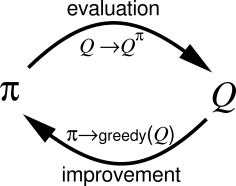
\includegraphics[scale=0.7]{figures/evalctrl.png}
          \caption{The alternation between evaluation and control}
          \label{fig:evalctrl}
        \end{figure}

        The second and the most widely used approach is called \textit{Temporal Difference Learning} (TD-Learning). The algorithms that belong to this category do not wait for the end of the episode to update the Q-function like in the case of Monte-Carlo, instead, they use other estimated values for other states and other actions; this is known as \textit{bootstraping}. The most famous TD algorithms are \textit{sarsa} and Q-Learning. The first one updates $Q(s_t,a_t)$ at time $t$ by choosing the next action given a policy derived from Q ($\epsilon$-greedy for example), obtaining an immediate reward $r_t$, moving to state $s_{t+1}$ and choosing $a_{t+1}$ using a policiy derived from Q again, then updating Q as follows ($\alpha$ being an update parameter):

            $$ Q(s_t,a_t) = Q(s_t,a_t) + \alpha [r_t + \gamma Q(s_{t+1},a_{t+1}) - Q(s_t,a_t)] $$

        %HK> Une référence pour sarsa?
        The idea behind this way of bootstrapping is that the Q is updated at each step by considering that it will follow a policy derived from Q during the next steps; this is an \textit{on-policy} algorithm. On the contrary, Q-Learning \cite{Watkins1989} is an \textit{off-policy} algorithm as it directly estimates $Q^*$ by performing the following update at each step:

            $$ Q(s_t,a_t) = Q(s_t,a_t) + \alpha [r_t + \gamma \max_a Q(s_{t+1},a_{t+1}) - Q(s_t,a_t)] $$


    \subsection{Application to dialogue systems}
    
    	Reinforcement learning has been first applied to dialogue systems in \cite{Levin1997} and since then, it has the leading machine learning framework in the field. The dialogue state at time $t$ is generally determined by the history of dialogue acts since the beginning of the dialogue. At each turn, the set of actions is made of all the possible answer at that time. Partially Observable Markov Decision Processes (POMDPs) are also widely used. In this framework, the dialogue state is replaced by a distribution over all possible states which is a more natural way of modeling uncertainty, however, they are more complex and more difficult to scale \cite{Lemon2007}.
        
        % Citer un maximum de papiers après Meena2013, notamment Turn-Yielding cues qui a cité Beatie1982.
        In the field of incremental dialogue and turn-taking management, supervised learning is more common. The main problem tackled by researchers is the identification of the exact moments where the system should take the floor in order to achieve smooth turn-taking \cite{Raux2008,Meena2013}. Binary classifiers are used and the features they are fed are of different natures: lexical, semantic, prosodic...etc...However, a few papers tackled this problem by using reinforcement learning.
        
        \cite{Jonsdottir2008} used reinforcement learning while considering prosodic features only. Backchanneling for example can be performed by humans independently from the meaning. The cost function (negative reward) is taken as gaps and overlaps, hence following Sack's principle discussed in Section \ref{soa:ttphuman}.
        
        \cite{Dethlefs2012} adopted a complementary approach where only the semantic content of the user's utterance is taken into account (hierarchical reinforcement learning is used). In human conversation, it is more likely for the listener to react right after a relevant information. Similarly, in the case of a restaurant finding spoken dialogue system, the system should react right after understanding the restaurant's type or price range. In this work, the information pertinence is measured by the Information Density (ID). Therefore, the more the ID is high during system actions, the more reward it gets.
        
        Instead of trying to minimise gaps and overlaps, the reward function can be designed in a way to optimise dialogue duration and task completion like it is the case in \cite{Selfridge2010}. The system in this paper learns optimal initial turn-taking, in the sense that when a silence is detected, the dialogue participant that has the most relevant thing to say takes the floor first. Like in the previous paper, only semantic features are considered.
        
        A third approach to optimise turn-taking in spoken dialogue systems is to directly try to imitate human behaviours. In \cite{Kim2014} Inverse Reinforcement Learning is used to infer a reward function directly from user trajectories in a gathered dialogue corpus. Therefore, the reward function automatically incorporates objective and subjective dialogue quality criteria. The authors have made the choice not to consider lexical and semantic features, but rather to limit their work to timing and prosody signals.
    
    \subsection{Dialogue simulation}
    
    	A couple of decades ago, as dialogue systems started to become a popular research fields, the need for evaluation means in order to assess their quality started getting more and more important. Therefore, researchers turn to user simulation methods (also referred to as user modeling). In \cite{Eckert1997}, some of the advantages of these techniques are depicted: reduced cost with automatic evaluation of a large number of dialogues, less error risk, easy modeling of different user populations, possibility of using the same user model across different concurrent dialogue systems for comparison and providing a tool to quickly generate corpora for machine learning techniques at a low cost. Nevertheless, the authors recognise that user simulation cannot totally replace interactions with real users in the process of designing reliable dialogue systems: \textit{However, we believe that tests with human users are still vital for verifying the simulation models.}.
        
       	Simulating users accurately is a challenging task as their behaviours vary considerably from a person to another and moreover, the same user can change her preferences over time (concept-drift) \cite{Schatzmann2006}. Evaluating a user simulator and whether it handles such variability or not is a research track in itself \cite{Pietquin2013} and the qualities required are of different kinds. The trained user simulator should be consistent with the data that has been used for the training and the sequence of dialogue acts generated should be coherent. In addition, when it is used in turn to train a data-driven dialogue strategy, the quality of the latter is also an evaluation criteria. Also, it is important that the results obtained in simulation give strong indications about the behaviours with real users while being task independent and automatically able to automatically compute assessments.
        
        User simulation is useful during the conception phase of a dialogue system. However, training the simulator from data needs the dialogue system to be conceived already. Therefore, trying to come up with a simple model with only a few parameters is not always a bad idea as it has been proven to achieve good results as well \cite{Schatzmann2007}.
        
        %HK> Citer paradise après la liste des KPIs pour la reward function
        User simulator is also quite similar to the dialogue management task. As a consequence, it is legitimate to ask the following question: why not use reinforcement learning to train user simulators? The answer is that in the case of dialogue management, it is easier to come up with a reasonable reward function: task completion, dialogue duration, subjective evaluation...etc... When it comes to user simulation, the objective function is how well a real user is imitated which is impossible to handcraft. Fortunately, there exists a framework where the reward function is automatically inferred from data which is particularly useful here: inverse reinforcement learning \cite{Chandramohan2011}.
        
        When it comes to incremental dialogue systems, the only existing user simulator in our knowledge is the one described in \cite{Selfridge2012b}. Its state is update every 10 ms. However, the \textit{ASR instability} phenomenon is not replicated, that is to say that the ASR hypothesis construction is monotonous whereas in reality, it is not the case. When a new audio signal increment is heard by the ASR, the output can be partially or totally modified. In this simulator, only the simple case where a new increment is added to the output is modeled.

\section{Issues and motivation}
    
    A study led by the Market Intelligence and Consulting Institute shows that the market of artificial intelligence should grow exponentially in the next decade. Virtual assistants play the main role in this domain and they are predicted to multiply their market share by 2.5. Moreover, the market is expected to multiply its turn over by 14 (30\% growth per year on average). This shows that SDSs have reached a level of maturity that enables them to significantly interest the market. Therefore, designing robust, reliable and user-friendly spoken dialogue systems raises an important issue.
    
    Nevertheless, even though virtual assistants like Siri or other more domain specific spoken dialogue systems can offer a quite reasonable quality of service for certain tasks, the quality of the interaction is still poor, making room for improvement in different areas:
    
    % HK> Rajouter une citation pour les erreurs d'ASR et la gestion des erreurs.
    \begin{itemize}
    	\item The ASR module is not perfect and the errors that it engenders are not well handled by the DM.
        \item The vocabulary is very restrained hence users often use off-domain words, especially those who are not familiar with the system.
        \item Current Natural Language Processing (NLP) techniques still do not cover a lot of discourse formulations, therefore NLU modules are often too simple to handle all the situations encountered in real dialogue.
        \item Current SDSs do not adapt to the user's profile neither to groups of users' particular behaviours (accent, culture, specific expressions...).
        \item Turn-taking is handled in a walkie-talkie manner which is too simple compared to the reality of dialogue.
    \end{itemize}
    
    In this thesis we focus on the last point: turn-taking capabilities improvement. We identified two research streams:
    
    %HK> Revoir les papiers de références ici et bien les placer.
    \begin{enumerate}
    	\item Barge-in points identification to achieve smoother and more human like turn-taking. When a barge-in point is detected, it can be interpreted as an end-point so that the system can take the floor in a more reactive way, or as a suitable point for backchanneling. In these kind of studies, prosodic features are crucial but they can also be mixed with lexical and semantic ones.
        \item Turn-taking optimisation to improve dialogue efficiency (generally measured through dialogue duration and task completion). The main objective is to improve error handling by reporting errors quickly, and to improve reactivity in general as the system can respond as soon as it has enough information to do so. Unlike the previous stream, semantic features have more importance here.
    \end{enumerate}
    
    This thesis is a contribution to the second research stream. First we try to understand what is turn-taking in human-human interaction, then we ask ourselves what phenomena can be replicated in human-machine dialogue in order to offer a better error-handling and an increased efficiency in general.
    
    
    
    
    
    

